%%% LaTeX Template: Article/Thesis/etc. with colored headings and special fonts
%%%
%%% Source: http://www.howtotex.com/
%%% Feel free to distribute this template, but please keep to referal to http://www.howtotex.com/ here.
%%% February 2011
%%%
%%% Modified October 2015 by CDM

%%%  Preamble
\documentclass[11pt,letterpaper]{article}
\usepackage[margin=1.0in]{geometry}
\usepackage[T1]{fontenc}
\usepackage[bitstream-charter]{mathdesign}
\usepackage[latin1]{inputenc}					
\usepackage{amsmath}						
\usepackage{xcolor}
\usepackage{cite}
\usepackage{hyphenat}
\usepackage{graphicx}
\usepackage{float}
\usepackage{subfigure}
\usepackage{sectsty}
\usepackage[compact]{titlesec} 
\usepackage[tablegrid]{vhistory}
\allsectionsfont{\color{accentcolor}\scshape\selectfont}

%%% Definitions
\definecolor{accentcolor}{rgb}{0.0,0.0,0.5} 
\newcommand{\teamname}{Team Tassium}
\newcommand{\productname}{Intelligrip}
\newcommand{\coursename}{CSE 4316: Senior Design I}
\newcommand{\semester}{Fall 2017}
\newcommand{\docname}{System Requirements Specification}
\newcommand{\department}{Department of Computer Science \& Engineering}
\newcommand{\university}{The University of Texas at Arlington}
\newcommand{\authors}{Anthony Tatowicz \\ Jesse Daniel Mitchell \\ Todd Brewer\\ Linh Vu}

%%% Headers and footers
\usepackage{fancyhdr}
	\pagestyle{fancy}						% Enabling the custom headers/footers
\usepackage{lastpage}	
	% Header (empty)
	\lhead{}
	\chead{}
	\rhead{}
	% Footer
	\lfoot{\footnotesize \teamname \ - \semester}
	\cfoot{}
	\rfoot{\footnotesize page \thepage\ of \pageref{LastPage}}	% "Page 1 of 2"
	\renewcommand{\headrulewidth}{0.0pt}
	\renewcommand{\footrulewidth}{0.4pt}

%%% Change the abstract environment
\usepackage[runin]{abstract}			% runin option for a run-in title
%\setlength\absleftindent{30pt}			% left margin
%\setlength\absrightindent{30pt}		% right margin
\abslabeldelim{\quad}	
\setlength{\abstitleskip}{-10pt}
\renewcommand{\abstractname}{}
\renewcommand{\abstracttextfont}{\color{accentcolor} \small \slshape}	% slanted text

%%% Start of the document
\begin{document}

%%% Cover sheet
{\centering \huge \color{accentcolor} \sc \textbf{\department \\ \university} \par}
\vspace{1 in}
{\centering \huge \color{accentcolor} \sc \textbf{\docname \\ \coursename \\ \semester} \par}
\vspace{0.5 in}
\begin{figure}[h!]
	\centering
   	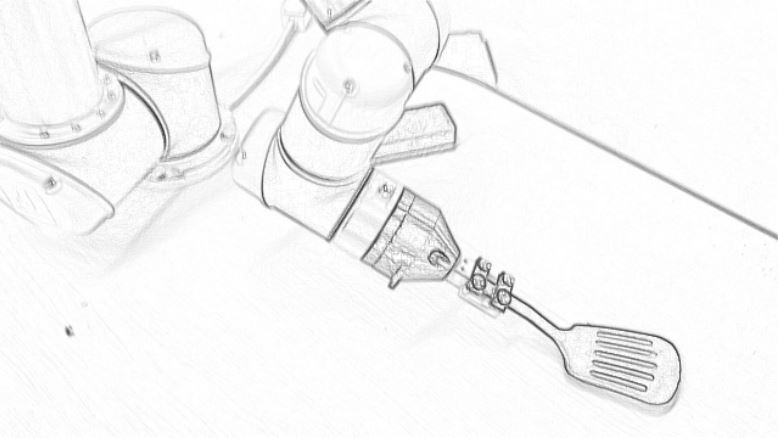
\includegraphics[width=0.60\textwidth]{images/test_image}
\end{figure}
\vspace{0.5 in}
{\centering \huge \color{accentcolor} \sc \textbf{\teamname \\ \productname} \par}
\vspace{0.5 in}
{\centering \large \sc \textbf{\authors} \par}
\newpage


%\vspace{1 in}
%\centerline{January 13th, 2012}
%\newpage

%%% Revision History
\begin{versionhistory}
  	\vhEntry{0.1}{10.27.2017}{LV}{First draft of contents 7,8,9}
\end{versionhistory}
\newpage

%%% Table of contents
\setcounter{tocdepth}{2}
\tableofcontents
\newpage

%%% List of figures and tables (optional)
\listoffigures
%\listoftables
\newpage

\section{Product Concept}
The application of the UR5 known as \productname{} is designed to reduce the cost of owning a business oriented around preparing food. With the increase in demand towards a higher minimum wage, many businesses will be seeking options to save money.

\subsection{Purpose and Use}
\productname{} will be able to prepare food (specifically hamburgers) to serve to a consumer. You will be able to queue up requests and receive the food.  

\subsection{Intended Audience}
The target audience for \productname{} are restaurant owners (more specifically ones that run chain restaurants), as \productname{} will allow them to save money on hiring workers.

This will allow owners to save money, worry less about payroll taxes, and serve quality food at a lower cost.

\begin{figure}[h!]
	\centering
   	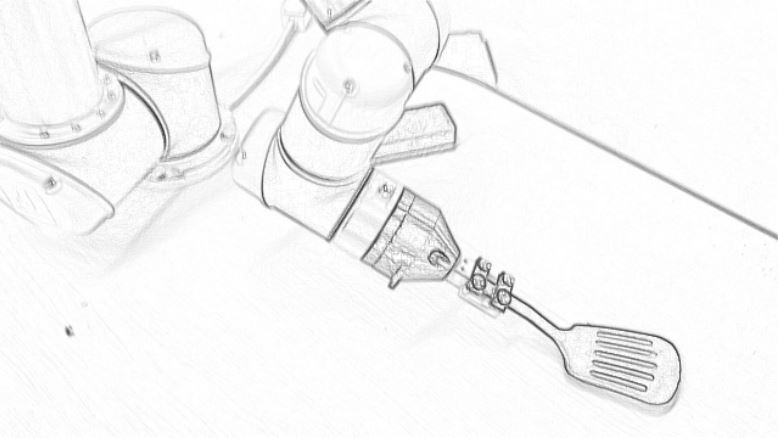
\includegraphics[width=0.60\textwidth]{images/test_image}
    \caption{X conceptual drawing}
\end{figure}

\newpage
\section{Product Description}
This section provides the reader with an overview of \productname{}, and the primary operational aspects of the product.

\subsection{Features \& Functions}

This product will cook hamburgers on the grill using vision processing, 3D Printed Mounts, the UR5 Robotic Arm, and a small grill. You will be able to queue up jobs for the \productname{} for it to know when to start cooking. 

It will specifically have a webcam, and various 3D Printed attachments. External equipment may also be designed to make it more convenient for the robot to finish preparing the burger. 

\subsection{External Inputs \& Outputs}
The product will receive basic instructions from a cashier, and also use a webcam to process where hamburger patties are. 

This webcam will allow it to instruct the webcam to pick up patties and move it onto the grill. Once it is done grilling, it will move it to a "finished" zone, and display a message that the hamburger is done. 


\subsection{Product Interfaces}
There will be a user interface designed to make it easy to queue up different hamburgers with assorted requirements (like if this burger have ketchup added on top). 

Aside from that, the product will be fairly autonomous. 
\newpage
\section{Customer Requirements}
It is important for the user to perform a risk assessment when using this product. Refer to the UR5 user manual for additional detailed specifications and requirements of the product's hardware. 

\subsection{Workspace Assessment}
\subsubsection{Description}
The UR5 must be used in a workspace within a radius of 850mm of the base. For all required functions, the tools and and attachments can only be used within this space. 

The UR5 has a maximum payload of 11 pounds so we must keep that in mind when assigning tasks.
\subsubsection{Priority}
Medium

\subsection{Tool and Attachment Bindings}
\subsubsection{Description}
Any tool or removable attachment secured to the mount of the UR5 must go through a safety check to ensure that the tool is secured and will not move within the mount while in use. This is to ensure the integrity and safety of the system.
\subsubsection{Priority}
High


\subsection{Ability to Prepare a Hamburger}
\subsubsection{Description}
The \productname{} should be able to prepare an edible hamburger to completion. 
\subsubsection{Standards}
- The burger patty must be cooked well-done. While steak is safe to eat "rare", ground beef is not. 
- The burger patty must be placed onto a bun by the UR5.   
\subsubsection{Priority}
High

\newpage
\section{Packaging Requirements}
Product is handled as is.  No additional packaging protocol or concerns are needed for this product.

\subsection{Packaging}
\subsubsection{Description}
Handled as is.
\subsubsection{Source}
UR5 Team (Team Tassium)
\subsubsection{Constraints}
N/A
\subsubsection{Standards}
N/A
\subsubsection{Priority}
Low
\newpage
\section{Performance Requirements}
\productname{} is a technology based on the UR5 platform developed to cook food. Speed and performance is a concern. 

\subsection{Speediness of Food Preparation}
\subsubsection{Description}
Our technology must be able to cook a hamburger to completion within a reasonable amount of time.
\subsubsection{Constraints}
- How is the throughput required? patties/hr?\\
- Human interaction constraints and safety?\\
- Reliability? \\
- Productivity goals?
\subsubsection{Standards}
- Health/Safety standards\\
\subsubsection{Priority}
High



\newpage
\section{Safety Requirements}
The \productname{} involves use of heat and moving components. Safety must be taken into consideration during the development of this project.

\subsection{Proximity Sensors}
\subsubsection{Description}
With moving components at play, it might be wise to install proximity sensors or at least a barrier to prevent a person from being struck with a moving component.
\subsubsection{Standards}
- Must prevent a person from being hit with the moving UR5.
\subsubsection{Priority}
Low. The UR5 moves slowly in its current state.



\subsection{Heat Safety}
\subsubsection{Description}
The UR5 and its attached components will interact with a griddle. We will need to ensure that our equipment is not damaged by the heat, and that we wear proper equipment to handle the heated components.
\subsubsection{Standards}
- Oven mitts or protective gloves must be worn when interacting with the grill.
- The equipment must not be in close proximity to any heat sources, at least not for very long. 
\subsubsection{Priority}
High
\newpage
\section{Maintenance \& Support Requirements}
The user of the product will be responsible for maintaining the product by troubleshooting with the manuals. If it is a hardware failures, the customer should contact the manufacturer(UR5). Any such requirement will be describe here in this section in details.

\subsection{Requirement Name}
Tools Maintenance
\\Software updates
\\User manual/support
\subsubsection{Description}
To be describe in the future
\subsubsection{Source}
Linh Vu
\subsubsection{Constraints}
None at this time
\subsubsection{Standards}
None at this time
\subsubsection{Priority}
Tools Maintenance: Moderate
\\Software updates : Moderate
\\User manual/support: Moderate
\newpage
\section{Other Requirements}
Items and tools that will be use in the final product will be describe here in this requirement section.

\subsection{Requirement Name}
Tool rack setup
\\Camera placement
\\UI
\subsubsection{Description}
Tool rack setup : Placement of the tool rack will be place at a specified position of the UR5.
\\Camera placement : Placement of a camera will be facing the UR5 at an angle and height for maximum visual.
\\UI : User interface that will allow the user to change the task of the UR5.
\subsubsection{Source}
Linh Vu
\subsubsection{Constraints}
Placement of the tool rack will be place at a specified position of UR5.
\subsubsection{Standards}
To be specified later.
\subsubsection{Priority}
Tool rack setup : Low
\\Camera placement : Low
\\UI : Low
\newpage
\section{Future Items}
All priority 5 in the previous section will be describe here in this section.

\subsection{Requirement Name}
\subsubsection{Description}
Detailed requirement description...
\subsubsection{Source}
Source
\subsubsection{Constraints}
Detailed description of applicable constraints...
\subsubsection{Standards}
List of applicable standards
\subsubsection{Priority}
Priority
\newpage

%%% References
\bibliographystyle{plain}
\bibliographystyle{reference/IEEEtran_custom}
\bibliography{reference/refs}{}

\end{document}